%% State Space Modelling of Dynamic Systems
%% Lecture 4: Time Response of a State-Space Model
\def\FileDate{98/10/14}
\def\FileVersion{1.0}
% ----------------------------------------------------------------
% Notes pages *********************************************************
% ----------------------------------------------------------------

Although a state-space model may uniquely represent a given
dynamic system, there is no state-space model that uniquely
represents a given transfer function. That is there are many
state-space models that can be transformed into a given transfer
function. If one begins the analysis of a dynamic system from an
analysis of the elementary dynamics then the state space model
that results from such an analysis will accurately reflect the
physical state variables in the system. However, if one's analysis
begins from a differential equation or (equivalently) from a
transfer function, then it is convenient to transform the model
description into one of a small number of ``standard'' or
\emph{canonical forms}.

\section*{The Companion Form}
These notes describe how a general differential equation may be
converted into a state-space model.

Consider the general differential equation:

\[
\frac{d^{n}y}{dt^{n}} +
a_{n-1}\frac{d^{n-1}y}{dt^{n-1}}+a_{n-2}\frac{d^{n-2}y}{dt^{n-2}}+\cdots+a_1\frac{dy}{dt}+a_0
y = b_0 u
\]
We rearrange this equation so that the highest power is on the
left
\[
\frac{d^{n}y}{dt^{n}} =
-a_{n-1}\frac{d^{n-1}y}{dt^{n-1}}-a_{n-2}\frac{d^{n-2}y}{dt^{n-2}}-\cdots-a_1\frac{dy}{dt}-a_0
y + b_0 u.
\]
Let:
\begin{eqnarray*}
x_1 &=& y \\ x_2 &=& \frac{dy}{dt} \\ x_3 & = & \frac{d^2y}{dt^2}
\\ \vdots \\ x_{n-1} &=& \frac{d^{n-2}y}{dt^{n-2}} \\ x_{n} &=& \frac{d^{n-1}y}{dt^{n-1}}
\end{eqnarray*}
If we differentiate both sides of these new definitions we obtain
\begin{eqnarray*}
\dot{x}_1 &=& \frac{dy}{dt} \\ \dot{x}_2 &=& \frac{d^2y}{dt^2} \\
\dot{x}_3 & = & \frac{d^3y}{dt^3}
\\ \vdots \\ \dot{x}_{n-1}  &=& \frac{d^{n-1}y}{dt^{n-1}} \\ \dot{x}_{n} &=& \frac{d^{n}y}{dt^{n}}
\end{eqnarray*}

These equations represent the left-hand-side of the state
equations and if we make the substitutions we get
\begin{eqnarray*}
\dot{x}_1 &=&
   x_2 \\ \dot{x}_2 &=&  x_3   \\
\dot{x}_3 & = &  x_4
\\ \vdots \\ \dot{x}_{n-1}  &=& x_n \\ \dot{x}_{n} &=&
-a_{0}x_1 -a_1x_2 - \cdots  -a_{n-2}x_{n-1} -a_{n-1}x_{n} + b_0 u
\end{eqnarray*}
We then define the state vector \[\mathbf{x}=[x_1,\ x_2,\ \ldots,\
x_n]^T\] and the matrix form of the state equations are
\[
\dot{\mathbf{x}} = \left[\begin{array}{ccccc}
  0 & 1 & 0 & \cdots & 0 \\
  0 & 0 & 1 & \cdots & 0 \\
  \vdots & \vdots & \vdots & \ddots & \vdots \\
  0 & 0 & 0 & \cdots & 1 \\
  -a_{0} & -a_{1} & -a_{2} & \cdots & -a_{n-1}
\end{array}\right]\mathbf{x}+\left[\begin{array}{c}
  0 \\
  0 \\
  0 \\
  \vdots \\
  1
\end{array}\right]u
\]
The system matrix is in ``\emph{companion form}'', so called because the
coefficients in the final row are the same as for the differential
equation. The output equation depends on the dependent variable of
interest but the simplest is $y=x_1$ which gives the solution of
the differential equation. Thus
\[y = [1,\ 0,\ 0,\ \ldots, 0] \mathbf{x}.\]

The transfer function equivalent of this differential equation is
obtained from the differential equation:
\[
\frac{d^{n}y}{dt^{n}} +
a_{n-1}\frac{d^{n-1}y}{dt^{n-1}}+a_{n-2}\frac{d^{n-2}y}{dt^{n-2}}+\cdots+a_1\frac{dy}{dt}+a_0
y = b_0 u
\]
The transform of this equation, ignoring initial conditions, is
\[
\left(s^n +
a_{n-1}s^{n-1}+a_{n-2}s^{n-2}+\cdots+a_1s+a_0\right)Y(s) = b_0
U(s)
\]
so the transfer function is
\[
G(s) = \frac{Y(s)}{U(s)} = \frac{b_0}{s^n +
a_{n-1}s^{n-1}+a_{n-2}s^{n-2}+\cdots+a_1s+a_0}.
\]
Note that the numerator has no terms in $s$. We shall consider
completely general case for both proper and strictly proper
systems later.

\section*{The Companion Form}

We have just shown that a state space model
for the system defined by the general differential equation, shown
in \sref{slide:l5s1}, was the companion form illustrated in
\sref{slide:l5s2}. This structure of this state-space model is
illustrated in \sref{slide:l5s3}.
\begin{slide}\label{slide:l5s1}
\heading{General Differential Equation}
\[ \frac{d^{n}y}{dt^{n}} +
a_{n-1}\frac{d^{n-1}y}{dt^{n-1}}+a_{n-2}\frac{d^{n-2}y}{dt^{n-2}}+\cdots+a_1\frac{dy}{dt}+a_0
y = b_0 u
\]
or transfer function
\[
G(s) = \frac{Y(s)}{U(s)} = \frac{b_0}{s^n +
a_{n-1}s^{n-1}+a_{n-2}s^{n-2}+\cdots+a_1s+a_0}.
\]
The state variables in this model are the so-called ``\emph{phase
variables}'' $x_1 = y$, $x_2 = dy/dt$, $\ldots$ $x_n = d^n/dt^n$.
\end{slide}
\begin{slide}\label{slide:l5s2}
\heading{Companion Form}
\begin{eqnarray*} \dot{\mathbf{x}} &=&
\left[\begin{array}{ccccc}
  0 & 1 & 0 & \cdots & 0 \\
  0 & 0 & 1 & \cdots & 0 \\
  \vdots & \vdots & \vdots & \ddots & \vdots \\
  0 & 0 & 0 & \cdots & 1 \\
  -a_{0} & -a_{1} & -a_{2} & \cdots & -a_{n-1}
\end{array}\right]\mathbf{x}+\left[\begin{array}{c}
  0 \\
  0 \\
  0 \\
  \vdots \\
  b_0
\end{array}\right]u\\
y & = & [1,\ 0,\ 0,\ \ldots, 0] \mathbf{x}.
\end{eqnarray*}
\end{slide}
\begin{slide}\label{slide:l5s3}
\heading{Block Diagram of Companion Form}
\resizebox{300pt}{!}{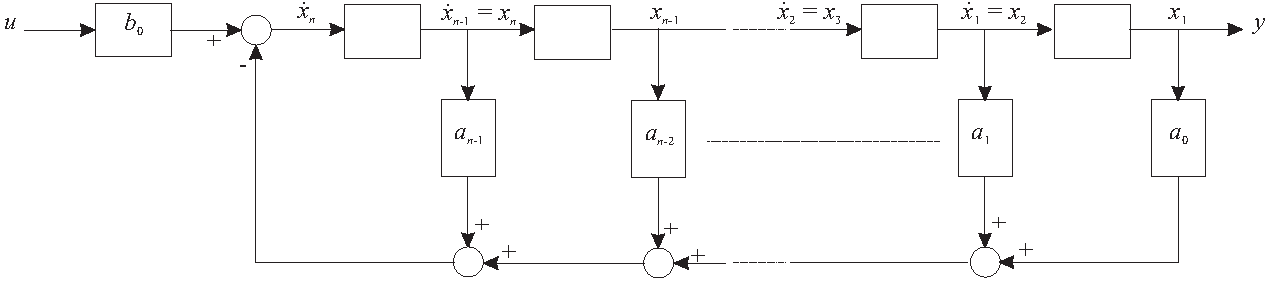
\includegraphics{pictures/companion1.eps}}
\end{slide}

Now let us consider the case of a system that has derivatives of
the input. A strictly proper system has transfer function
\[G(s)=\frac{Y(s)}{U(s)} = \frac{b_ms^m +
b_{m-1}s^{m-1}+b_{m-2}s^{m-2}+\cdots+b_1s+b_0}{s^n +
a_{n-1}s^{n-1}+a_{n-2}s^{n-2}+\cdots+a_1s+a_0}\] where $m<n$. How
is this more general system converted into a state-space model?
Well, from the previous result let us use the state definition
$x_1(t) = y(t)$ to split the transfer function so that
\begin{equation}\label{eq:l5e1}
X_1(s) = \frac{1}{s^n +
a_{n-1}s^{n-1}+a_{n-2}s^{n-2}+\cdots+a_1s+a_0}U(s)
\end{equation}
and
\begin{equation}\label{eq:l5e2}
Y(s) = \left(b_ms^m +
b_{m-1}s^{m-1}+b_{m-2}s^{m-2}+\cdots+b_1s+b_0\right)X_1(s).\end{equation}
Inverse Laplace transforming equation (\ref{eq:l5e2}) we get:
\begin{eqnarray}\label{eq:l5e3}
y(t) & = & b_m\frac{d^m}{dt^m}x_1(t) +
b_{m-1}\frac{d^{m-1}}{dt^{m-1}}x_1(t)+\cdots+b_1\frac{d}{dt}x_1(t)+
b_0x_1(t)\\ & = & b_mx_{m+1}(t) + b_{m-1}x_m(t)+\cdots+b_1x_2(t)+
b_0x_1(t).\label{eq:l5e4}
\end{eqnarray}
Where, in (\ref{eq:l5e4}), substitutions have been made according
to the definition of the phase variables. The vector state
equations are therefore: \begin{eqnarray*} \dot{\mathbf{x}} &=&
\left[\begin{array}{ccccc}
  0 & 1 & 0 & \cdots & 0 \\
  0 & 0 & 1 & \cdots & 0 \\
  \vdots & \vdots & \vdots & \ddots & \vdots \\
  0 & 0 & 0 & \cdots & 1 \\
  -a_{0} & -a_{1} & -a_{2} & \cdots & -a_{n-1}
\end{array}\right]\mathbf{x}+\left[\begin{array}{c}
  0 \\
  0 \\
  0 \\
  \vdots \\
  1
\end{array}\right]u\\
y & = & [b_0,\ b_1,\ \dots,\ b_{m-1}, b_m]
\mathbf{x}.\end{eqnarray*} Note that the coefficients of the
numerator appear in reverse order in the $\mathbf{C}$ matrix. The
structure of this system is illustrated in \sref{slide:l5s4} for
the case $m=n-1$.
\begin{slide}\label{slide:l5s4}
\heading{Strictly Proper Companion Form}
\resizebox{300pt}{!}{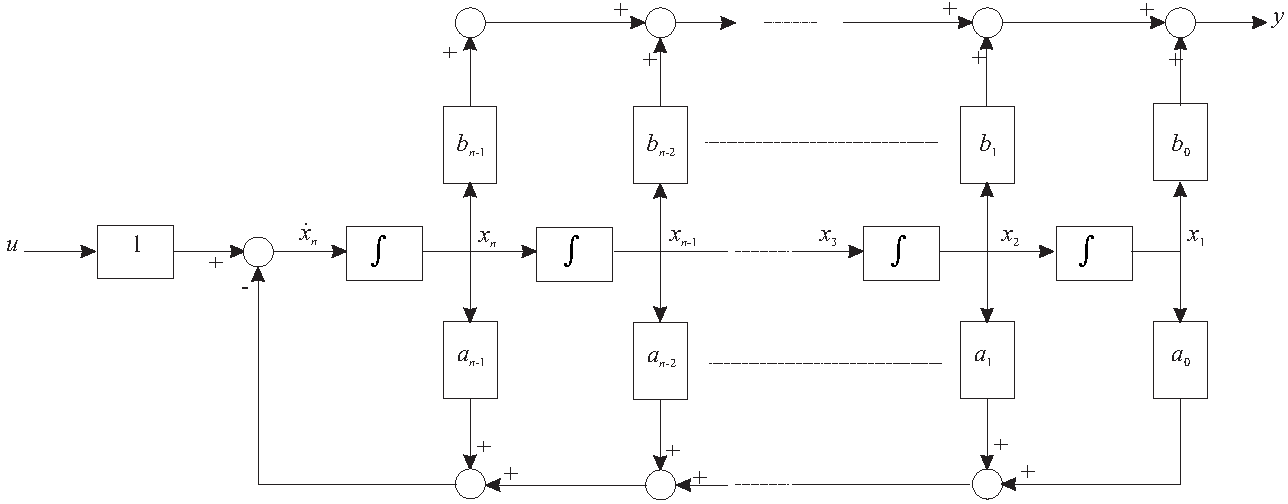
\includegraphics{pictures/companion2.eps}}
\end{slide}

The general form of a transfer function of a proper single-input,
single-output system of order $n$ is
\[\frac{b_ns^n+b_{n-1}s^{n-1}+\cdots+b_1s + b_0}{s^n+a_{n-1}s^{n-1}+\cdots+a_1s + a_0}\]
An alternative form, obtained by dividing the numerator by the
denominator, is
\[b_n+\frac{(b_{n-1}-b_n)s^{n-1}+\cdots+(b_1-b_n)+(b_0-b_n)}{s^n+a_{n-1}s^{n-1}+\cdots+a_1s + a_0}.\]
If we define $d=b_n$ and the modified numerator coefficients are
\[c_j=b_j-b_n,\ j=1,2,\ldots,n\] then the transfer function may be
re-written
\[d+\frac{c_{n-1}s^{n-1}+c_{n-2}s^{n-2}+\cdots+c_1s + c_n}{s^n+a_{n-1}s^{n-1}+\cdots++a_1s + a_0}.\]
Writing the transfer function in its functional form we have:
\[Y(s)=d U(s) +\frac{c_{n-1}s^{n-1}+c_{n-2}s^{n-2}+\cdots+c_1s +
c_n}{s^n+a_{n-1}s^{n-1}+\cdots+a_1s + a_0}U(s).\] Performing a
similar analysis, as before, we obtain the state-equations for a
proper system:
\begin{eqnarray*}\dot{\mathbf{x}} & = & \left[\begin{array}{ccccc}
  0 & 1 & 0 & \cdots & 0 \\
  0 & 0 & 1 & \cdots & 0 \\
  \vdots & \vdots & \vdots & \ddots & \vdots \\
  0 & 0 & 0 & \cdots & 1 \\
  -a_{0} & -a_{1} & -a_{2} & \cdots & -a_{n-1}
\end{array}\right]\mathbf{x}+\left[\begin{array}{c}
  0 \\
  0 \\
  0 \\
  \vdots \\
  1
\end{array}\right]u\\
y & = & [c_0,\ c_1,\ \dots,\ c_{m-1}, c_m] \mathbf{x} + d
u.\end{eqnarray*} The block diagram fro this system is illustrated
in \sref{slide:proper}.
\begin{slide}\label{slide:proper}
\heading{Proper System: Block Diagram}
\resizebox{320pt}{!}{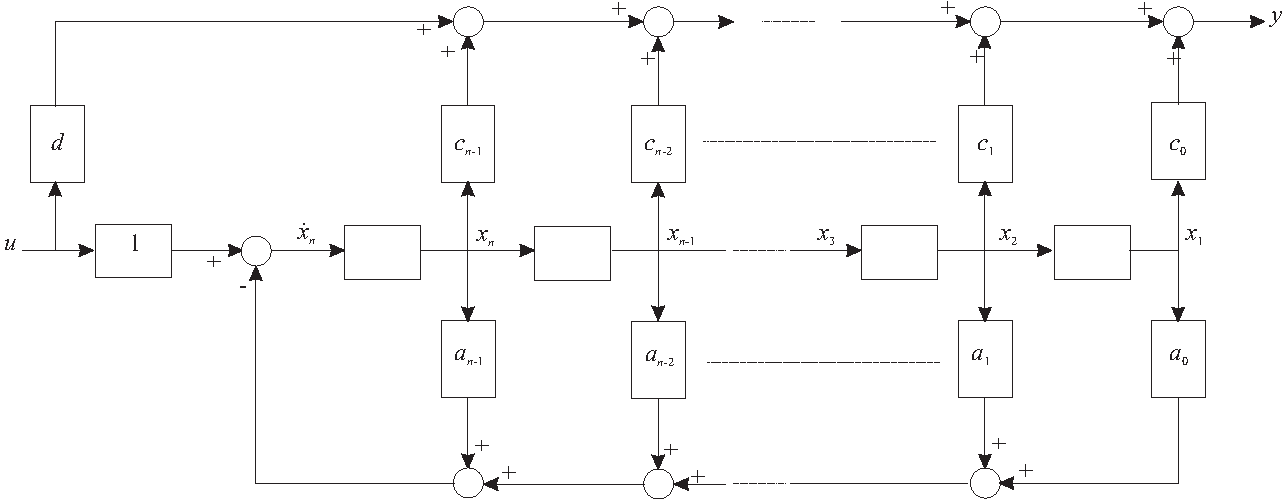
\includegraphics{pictures/companion3.eps}}
\end{slide}


\section*{Example}

\begin{slide}
\heading{Example}
System with transfer function
\[G(s)=\frac{Y(s)}{U(s)}=\frac{2s^3 + 16s^2 + 30s + 8}{s^3 + 7s^2 + 10s}\]
This system is ``proper'' because order of numerator equals order of denominator.
\end{slide}
\begin{slide}
\heading{Example (2)}
First divide the numerator into the denominator to get
\begin{eqnarray*}G(s)&=&\frac{2(s^3 + 7s^2 + 10s) + 2s^2 + 10s + 8}{s^3 + 7s^2 +
10s}\\ &=& \frac{2s^2 + 10s + 8}{s^3 + 7s^2 + 10s} +
2.\end{eqnarray*} 
\end{slide}
\begin{slide}
\heading{Example (completed)}
The companion form of the state matrices are
\begin{eqnarray*}\mathbf{A} & = & \left[\begin{array}{ccc}
  0 & 1 & 0 \\
  0 & 0 & 1 \\
  0 & -10 & -7
\end{array}\right]\ \mathbf{B}=\left[\begin{array}{c}
  0 \\
  0 \\
  1
\end{array}\right]\\ \mathbf{C} & = & \left[\begin{array}{ccc}
  8 & 10 & 2
\end{array}\right]\ \mathbf{D}=\left[2\right]\end{eqnarray*}
\end{slide}



%----------------------------------------------------------------
% The end of notes
% ----------------------------------------------------------------
\endinput

%%% Local Variables: 
%%% mode: latex
%%% TeX-master: t
%%% End: 
